\documentclass[leqno]{article}
% Shared QBT/Soln pack preamble for resources.danieljsmith.org.
\usepackage{graphicx}
\usepackage{dsfont}
\usepackage{mathtools}
\usepackage{amssymb}
\usepackage{amsmath}
\usepackage{amsthm}
\usepackage{float}
\usepackage{ragged2e}
\usepackage{tensor}
\usepackage{fancyhdr}
\usepackage{empheq}
\usepackage[most]{tcolorbox}
\usepackage{enumitem}
\usepackage{dirtytalk}
\usepackage{marginnote}
\usepackage{microtype}
\usepackage[
  a4paper,
  left=0.8in,
  right=1in,
  top=1in,
  bottom=0.5in,
  headheight=14pt,
  headsep=0.4in
]{geometry}
\setlength{\parindent}{0cm}

% TikZ / PGFPlots
\usepackage{pgfplots}
\pgfplotsset{compat=1.18}
\usepgfplotslibrary{fillbetween, polar}
\usetikzlibrary{calc, positioning}
\usetikzlibrary{angles, quotes}
\usetikzlibrary{arrows.meta}
\usetikzlibrary{decorations.pathreplacing, decorations.markings}
\usetikzlibrary{patterns}
\usetikzlibrary{intersections}

% Links and contents
\usepackage[colorlinks=true,linkcolor=black,citecolor=magenta,urlcolor=black]{hyperref}%
\urlstyle{same}

% Pack macros
\RenewDocumentCommand{\marks}{o m}{%
  \IfValueTF{#1}%
    {\marginnote{\raggedright\textbf{[#2]}}[#1]}%
    {\marginnote{\raggedright\textbf{[#2]}}}%
}

\newcommand{\vspacerule}[2]{%
  \par\vspace*{#1}%
  \noindent\hrulefill\par
  \vspace*{#2}%
}

\definecolor{scarlet}{RGB}{205, 40, 75}

% Worked-solution box, adapted from the TMUA worked-solutions box. A white breakable box with a left scarlet rule and no surrounding
% frame or tint. A part that breaks fills the rest of its page, so the rule
% runs to the bottom margin; the unbroken or last part ends in a short
% horizontal foot rule so a solution visibly stops. Unlike the TMUA box there
% is no answer label and no extra \parskip: these solutions mix \\ line breaks
% with blank lines, so paragraph skips would make the spacing uneven. The box
% does not grow to the left, so the rule sits at the text edge; growing to the
% right keeps the usable line width close to the old tcolorbox Solution box.
\newtcolorbox{djsSolution}{%
  enhanced, breakable, frame hidden, sharp corners, colback=white,
  height fixed for=first and middle, height fill,
  extras unbroken and last={natural height},
  borderline west={2.2pt}{0pt}{scarlet},
  left=11pt, right=0pt, top=5pt, bottom=13pt,
  before skip=13pt, after skip=4pt,
  grow to right by=10mm,
  overlay unbroken and last={%
    \fill[scarlet] (frame.south west)
      rectangle ([xshift=3.5cm, yshift=2.2pt]frame.south west);},
  before upper={{\color{scarlet}\bfseries Solution}\par\vspace{4pt}}}

% Optional smaller figure inside a solution box. \scalebox shrinks node text
% with the drawing. Not applied to existing figures.
\newcommand{\SolnFigureScale}{0.85}
\newsavebox{\djsSolnFigureBox}
\newenvironment{djsSolutionFigure}
  {\par\vspace{4pt}\begin{center}\begin{lrbox}{\djsSolnFigureBox}}
  {\end{lrbox}\scalebox{\SolnFigureScale}{\usebox{\djsSolnFigureBox}}%
   \end{center}\vspace{2pt}\par}

\newcommand{\cxl}[2]{%
  \tikz[baseline=(X.base)]{%
    \node[inner sep=0pt, outer sep=0pt, text=#1] (X) {$#2$};
    \draw[#1, line width=0.4pt] (X.south west)--(X.north east);
  }%
}

% Page-style hook run at the contents page and each question's opening page.
% A no-op for QBT packs; \djsSolnHeader points it at the fancy header.
\newcommand{\djsQuestionPageStyle}{}

\newcommand{\questionitem}{%
  \djsQuestionPageStyle
  \item\phantomsection
  \addcontentsline{toc}{section}{Question \number\value{enumi}}%
}

\renewcommand{\contentsname}{Questions}

\newcommand{\djsPackHeader}[1]{%
  \pagestyle{fancy}%
  \fancyhead{}%
  \fancyfoot{}%
  \renewcommand{\headrulewidth}{0.9pt}%
  \lhead{#1}%
  \chead{}%
  \rhead{\href{https://danieljsmith.org}{danieljsmith.org}}%
}

\newcommand{\djsQbtHeader}[1]{%
  \djsPackHeader{#1}%
}

% Solutions packs show the header only on the contents page and each
% question's opening page, so it never appears part-way through a solution.
% \thispagestyle marks the next page shipped out, which is the question's
% page because every solution question starts after a \newpage.
\newcommand{\djsSolnHeader}[1]{%
  \djsPackHeader{\textit{Solutions} - #1}%
  \pagestyle{empty}%
  \renewcommand{\djsQuestionPageStyle}{\thispagestyle{fancy}}%
}

\newcommand{\djsFrontMatter}{%
  \djsQuestionPageStyle
  \vspace*{20pt}%
  \tableofcontents
  \newpage
}


\djsQbtHeader{Centre of Mass of Polygonal Laminae}

\begin{document}
\djsFrontMatter
\begin{enumerate}[
  label=\textbf{\arabic*.},
  leftmargin=*,
  topsep=0pt,
  partopsep=0pt,
  parsep=0pt
]

% ---- Question 1 ----
\questionitem
% [Source: _QBT__Centre_of_Mass_of_Polygonal_Laminae, Q1]

\begin{figure}[H]
    \centering
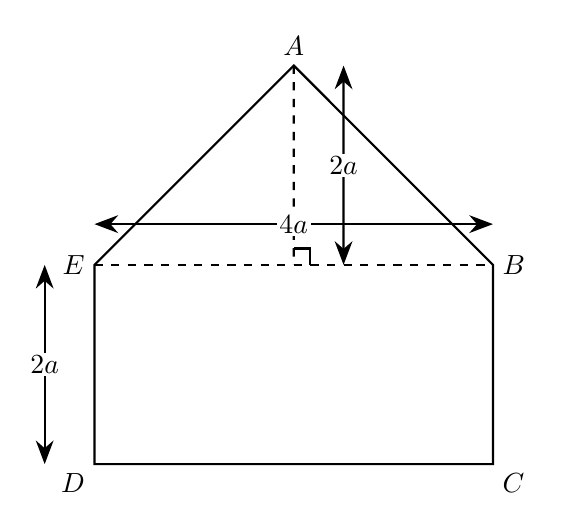
\begin{tikzpicture}[scale=1.15]
\def\a{1.1}
\coordinate (D) at (0,0);
\coordinate (C) at ({4*\a},0);
\coordinate (E) at (0,{2*\a});
\coordinate (B) at ({4*\a},{2*\a});
\coordinate (M) at ($(E)!0.5!(B)$);
\coordinate (A) at ($(M)+(0,{2*\a})$);

\draw[thick] (A) -- (B) -- (C) -- (D) -- (E) -- cycle;
\draw[dashed, thick] (E) -- (B);
\draw[dashed, thick] (A) -- (M);
\draw[thick] ($(M)+(0,0.18)$) -- ($(M)+(0.18,0.18)$) -- ($(M)+(0.18,0)$);

\draw[{Stealth[length=3mm]}-{Stealth[length=3mm]}, thick]
    ($(E)+(0,0.45)$) -- node[midway, fill=white, inner sep=1pt] {$4a$} ($(B)+(0,0.45)$);
\draw[{Stealth[length=3mm]}-{Stealth[length=3mm]}, thick]
    ($(D)+(-0.55,0)$) -- node[midway, fill=white, inner sep=1pt] {$2a$} ($(E)+(-0.55,0)$);
\draw[{Stealth[length=3mm]}-{Stealth[length=3mm]}, thick]
    ($(M)+(0.55,0)$) -- node[midway, fill=white, inner sep=1pt] {$2a$} ($(A)+(0.55,0)$);

\node[above] at (A) {$A$};
\node[right] at (B) {$B$};
\node[below right] at (C) {$C$};
\node[below left] at (D) {$D$};
\node[left] at (E) {$E$};
\end{tikzpicture}
\end{figure}


A uniform plane lamina is in the shape of the pentagon $ABCDE$, as shown shaded in the diagram above. \\
\begin{itemize}
  \item $BCDE$ is a rectangle
  \item $BE=4a$ and $DE=2a$
  \item triangle $ABE$ is isosceles with perpendicular height $2a$
\end{itemize}
\begin{enumerate}[label=\textbf{(\alph*)}]
  \item Show that the distance of the centre of mass of the lamina from $CD$ is $\dfrac{14a}{9}$. \marks{5} \\
\end{enumerate}
The mass of the lamina is $M$. \\

The lamina is suspended by two light vertical strings, one attached to the lamina at $D$ and the other attached to the lamina at $E$. \\

The lamina hangs freely in equilibrium, with $DE$ horizontal. \\
\begin{enumerate}[label=\textbf{(\alph*)}, resume]
  \item Using part (a), find, in terms of $M$ and $g$, the tension in the string attached at $E$. \marks{2} \\
\end{enumerate}


\newpage

% ---- Question 2 ----
\questionitem
% [Source: _QBT__Centre_of_Mass_of_Polygonal_Laminae, Q2]

\begin{figure}[H]
    \centering
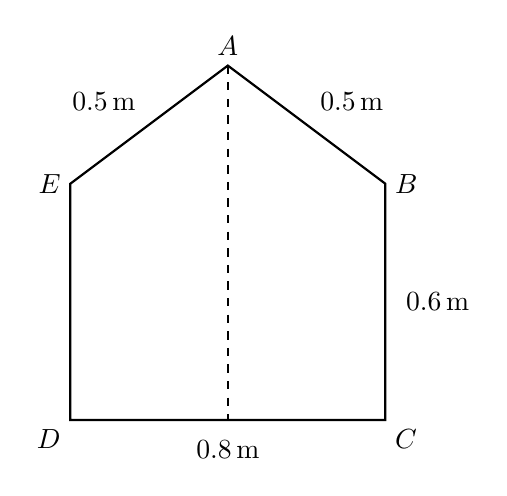
\begin{tikzpicture}[scale=5]
\def\w{0.8}
\def\h{0.6}
\def\roofside{0.5}
\pgfmathsetmacro{\halfw}{\w/2}
\pgfmathsetmacro{\roofh}{sqrt(\roofside*\roofside-\halfw*\halfw)}

\coordinate (D) at (-\halfw,0);
\coordinate (C) at (\halfw,0);
\coordinate (E) at (-\halfw,\h);
\coordinate (B) at (\halfw,\h);
\coordinate (A) at (0,{\h+\roofh});
\coordinate (M) at ($(C)!0.5!(D)$);

\draw[thick] (A) -- (B) -- (C) -- (D) -- (E) -- cycle;
\draw[dashed, thick] (A) -- (M);

\node[above] at (A) {$A$};
\node[right] at (B) {$B$};
\node[below right] at (C) {$C$};
\node[below left] at (D) {$D$};
\node[left] at (E) {$E$};

\node[above right=2pt] at ($(A)!0.5!(B)$) {$0.5\,\mathrm{m}$};
\node[above left=2pt] at ($(A)!0.5!(E)$) {$0.5\,\mathrm{m}$};
\node[right=4pt] at ($(B)!0.5!(C)$) {$0.6\,\mathrm{m}$};
\node[below=4pt] at ($(C)!0.5!(D)$) {$0.8\,\mathrm{m}$};
\end{tikzpicture}
\end{figure}


$ABCDE$ is a uniform lamina formed by joining an isosceles triangle $ABE$ to the top of a rectangle $BCDE$, where $AB=AE=0.5\,\mathrm{m}$, $BC=DE=0.6\,\mathrm{m}$ and $CD=BE=0.8\,\mathrm{m}$, as shown in the diagram. The centre of mass of the lamina is $G$. \\
\begin{enumerate}[label=\textbf{(\alph*)}]
  \item Explain why $G$ lies on the dashed line. \marks{1} \\
  \item Show that the perpendicular distance of $G$ from $CD$ is $0.38\,\mathrm{m}$. \marks{4} \\
\end{enumerate}
The lamina is freely suspended from the point $B$. \\
\begin{enumerate}[label=\textbf{(\alph*)}, resume]
  \item Determine the acute angle that $CD$ makes with the horizontal, stating which of $C$ or $D$ is higher. \marks{4} \\
\end{enumerate}

\newpage

% ---- Question 3 ----
\questionitem
% [Source: _QBT__Centre_of_Mass_of_Polygonal_Laminae, Q3]

\begin{figure}[H]
    \centering
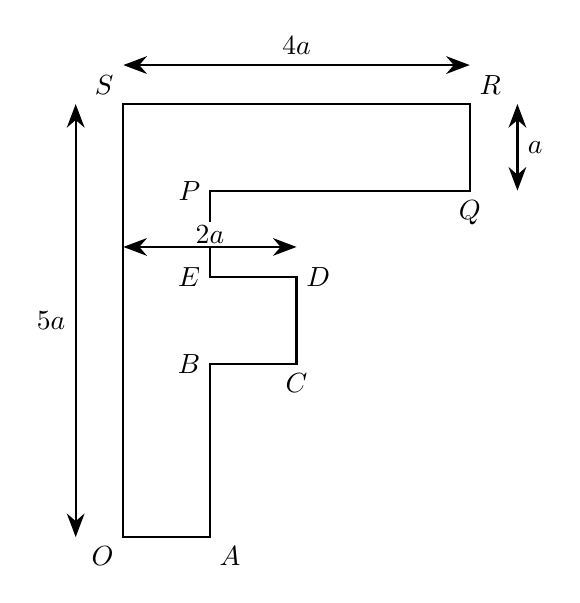
\begin{tikzpicture}[scale=1.0]
\def\a{1.1}

\coordinate (O) at (0,0);
\coordinate (A) at (\a,0);
\coordinate (B) at (\a,{2*\a});
\coordinate (C) at ({2*\a},{2*\a});
\coordinate (D) at ({2*\a},{3*\a});
\coordinate (E) at (\a,{3*\a});
\coordinate (P) at (\a,{4*\a});
\coordinate (Q) at ({4*\a},{4*\a});
\coordinate (R) at ({4*\a},{5*\a});
\coordinate (S) at (0,{5*\a});

\coordinate (V1) at ({-0.55*\a},0);
\coordinate (V2) at ({-0.55*\a},{5*\a});
\coordinate (H1) at (0,{5.45*\a});
\coordinate (H2) at ({4*\a},{5.45*\a});
\coordinate (M1) at (0,{3.35*\a});
\coordinate (M2) at ({2*\a},{3.35*\a});
\coordinate (T1) at ({4.55*\a},{4*\a});
\coordinate (T2) at ({4.55*\a},{5*\a});

\draw[thick] (O) -- (A) -- (B) -- (C) -- (D) -- (E) -- (P) -- (Q) -- (R) -- (S) -- cycle;

\draw[{Stealth[length=3mm]}-{Stealth[length=3mm]}, thick] (V1) -- (V2) node[midway,left] {$5a$};
\draw[{Stealth[length=3mm]}-{Stealth[length=3mm]}, thick] (H1) -- (H2) node[midway,above] {$4a$};
\draw[{Stealth[length=3mm]}-{Stealth[length=3mm]}, thick] (M1) -- (M2) node[midway,above,fill=white,inner sep=1pt] {$2a$};
\draw[{Stealth[length=3mm]}-{Stealth[length=3mm]}, thick] (T1) -- (T2) node[midway,right] {$a$};

\node[below left] at (O) {$O$};
\node[below right] at (A) {$A$};
\node[left] at (B) {$B$};
\node[below] at (C) {$C$};
\node[right] at (D) {$D$};
\node[left] at (E) {$E$};
\node[left] at (P) {$P$};
\node[below] at (Q) {$Q$};
\node[above right] at (R) {$R$};
\node[above left] at (S) {$S$};
\end{tikzpicture}
\end{figure}


A letter $F$ from a shop sign is modelled as a uniform plane lamina in the shape shown in the diagram above. \\

The left-hand vertical strip has width $a$ and height $5a$. The top horizontal strip has length $4a$ and thickness $a$. The middle horizontal strip has length $2a$ and thickness $a$. \\

Using the model, \\
\begin{enumerate}[label=\textbf{(\alph*)}]
  \item find, in terms of $a$, the distance of the centre of mass of the letter $F$, from
  \begin{enumerate}[label=(\roman*)]
    \item $OS$
    \item $OA$
  \end{enumerate}
  \marks{6}
\end{enumerate}
The letter $F$ is freely suspended from $O$ and hangs in equilibrium. The angle between $OS$ and the downward vertical is $\alpha$. \\

Using the model, \\
\begin{enumerate}[label=\textbf{(\alph*)}, resume]
  \item find the exact value of $\tan\alpha$. \marks{2} \\
\end{enumerate}

\newpage

% ---- Question 4 ----
\questionitem
% [Source: _QBT__Centre_of_Mass_of_Polygonal_Laminae, Q4]

\begin{figure}[H]
    \centering
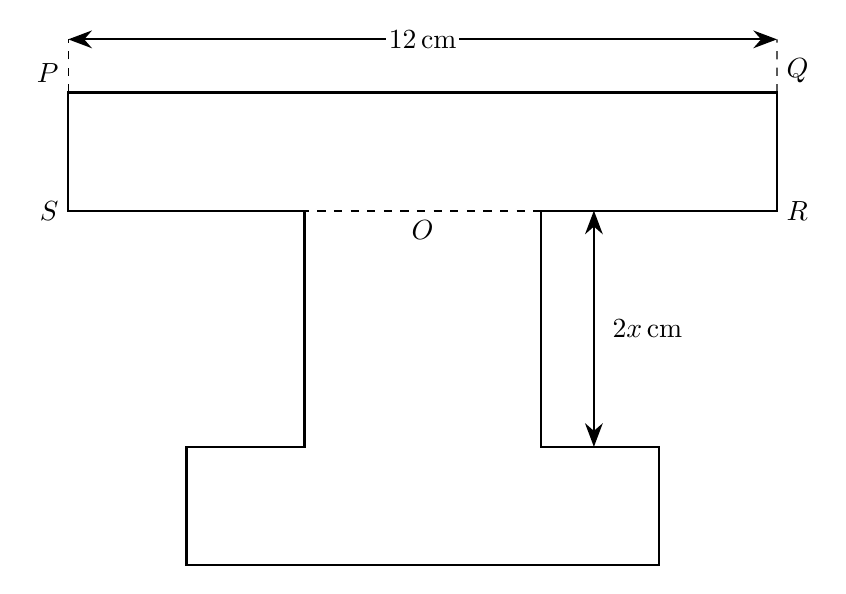
\begin{tikzpicture}[scale=0.75]
\def\Wtop{12}
\def\Hbar{2}
\def\Wstem{4}
\def\Wbot{8}
\def\Hbot{2}
\def\xshown{2}
\def\topoff{0.9}
\def\sideoff{0.9}
\pgfmathsetmacro{\Hstem}{2*\xshown}
\pgfmathsetmacro{\yref}{\Hbot+\Hstem}
\pgfmathsetmacro{\ytop}{\yref+\Hbar}
\pgfmathsetmacro{\xleftstem}{(\Wtop-\Wstem)/2}
\pgfmathsetmacro{\xrightstem}{(\Wtop+\Wstem)/2}
\pgfmathsetmacro{\xleftbot}{(\Wtop-\Wbot)/2}
\pgfmathsetmacro{\xrightbot}{(\Wtop+\Wbot)/2}

\coordinate (P) at (0,\ytop);
\coordinate (Q) at (\Wtop,\ytop);
\coordinate (R) at (\Wtop,\yref);
\coordinate (S) at (0,\yref);
\coordinate (O) at ($(S)!0.5!(R)$);
\coordinate (A) at (\xleftstem,\yref);
\coordinate (B) at (\xrightstem,\yref);
\coordinate (C) at (\xrightstem,\Hbot);
\coordinate (D) at (\xleftstem,\Hbot);
\coordinate (E) at (\xleftbot,\Hbot);
\coordinate (F) at (\xrightbot,\Hbot);
\coordinate (G) at (\xrightbot,0);
\coordinate (H) at (\xleftbot,0);
\coordinate (Pdim) at ($(P)+(0,\topoff)$);
\coordinate (Qdim) at ($(Q)+(0,\topoff)$);
\coordinate (Bdim) at ($(B)+(\sideoff,0)$);
\coordinate (Cdim) at ($(C)+(\sideoff,0)$);

\draw[dashed, thick] (S) -- (R);

\draw[thick]
  (P) -- (Q) -- (R) -- (B) -- (C) -- (F) -- (G) -- (H) -- (E) -- (D) -- (A) -- (S) -- cycle;

\draw[dashed] (P) -- (Pdim);
\draw[dashed] (Q) -- (Qdim);
\draw[{Stealth[length=3mm]}-{Stealth[length=3mm]}, thick]
  (Pdim) -- node[midway, fill=white, inner sep=1pt] {$12\,\mathrm{cm}$} (Qdim);

\draw[dashed] (B) -- (Bdim);
\draw[dashed] (C) -- (Cdim);
\draw[{Stealth[length=3mm]}-{Stealth[length=3mm]}, thick]
  (Cdim) -- node[midway, right=3pt] {$2x\,\mathrm{cm}$} (Bdim);

\node[above left] at (P) {$P$};
\node[above right] at (Q) {$Q$};
\node[right] at (R) {$R$};
\node[left] at (S) {$S$};
\node[below] at (O) {$O$};
\end{tikzpicture}
\end{figure}


A template $T$ consists of a uniform plane lamina made from three rectangles, as shown in the diagram. The upper rectangle $PQRS$ has $PQ=12\,\mathrm{cm}$ and $PS=2\,\mathrm{cm}$. The point $O$ is the midpoint of $SR$. A rectangle of width $4\,\mathrm{cm}$ and height $2x\,\mathrm{cm}$ is attached centrally below $SR$, and a rectangle of width $8\,\mathrm{cm}$ and height $2\,\mathrm{cm}$ is attached centrally below this rectangle. The whole template is symmetrical about the line through $O$ perpendicular to $SR$, where $x>1$. \\
\begin{enumerate}[label=\textbf{(\alph*)}]
  \item Show that the centre of mass of $T$ is a distance
  \[
  \dfrac{x^2+4x-1}{x+5}\,\mathrm{cm}
  \]
  below $SR$. \marks{7} \\
\end{enumerate}
The template $T$ is freely suspended from the point $P$ and hangs in equilibrium. \\

Given that $x=2$ and that $\theta$ is the angle that $PQ$ makes with the horizontal, \\
\begin{enumerate}[label=\textbf{(\alph*)}, resume]
  \item show that
  \[
  \tan\theta=\dfrac{42}{25}
  \]
  \marks[-20pt]{4}
\end{enumerate}


\newpage

% ---- Question 5 ----
\questionitem
% [Source: _QBT__Centre_of_Mass_of_Polygonal_Laminae, Q5]

\begin{figure}[H]
    \centering
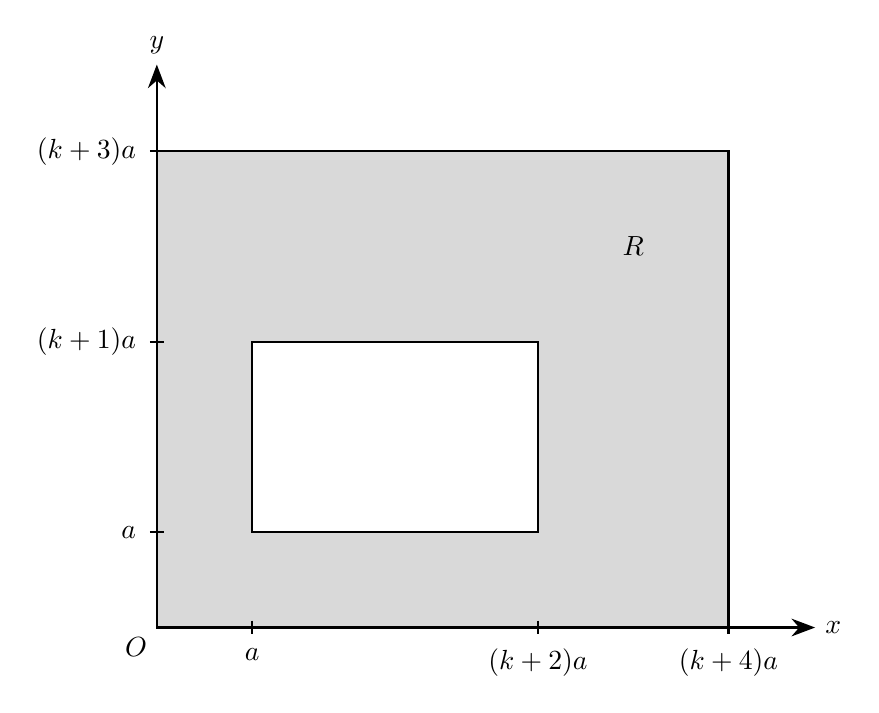
\begin{tikzpicture}[scale=1.1]
\def\alen{1.1}
\def\kval{2}
\pgfmathsetmacro{\xinnerL}{\alen}
\pgfmathsetmacro{\xinnerR}{(\kval+2)*\alen}
\pgfmathsetmacro{\xouter}{(\kval+4)*\alen}
\pgfmathsetmacro{\yinnerB}{\alen}
\pgfmathsetmacro{\yinnerT}{(\kval+1)*\alen}
\pgfmathsetmacro{\youter}{(\kval+3)*\alen}
\pgfmathsetmacro{\xmax}{\xouter+1.0}
\pgfmathsetmacro{\ymax}{\youter+1.0}

\coordinate (O) at (0,0);

\draw[-{Stealth[length=3mm]}, thick] (O) -- (\xmax,0) node[right] {$x$};
\draw[-{Stealth[length=3mm]}, thick] (O) -- (0,\ymax) node[above] {$y$};

\fill[gray!30, even odd rule] (0,0) rectangle (\xouter,\youter) (\xinnerL,\yinnerB) rectangle (\xinnerR,\yinnerT);
\draw[thick] (0,0) rectangle (\xouter,\youter);
\draw[thick] (\xinnerL,\yinnerB) rectangle (\xinnerR,\yinnerT);

\node[below left] at (O) {$O$};
\node at ({(\xinnerR+\xouter)/2},{(\yinnerT+\youter)/2}) {$R$};

\foreach \x in {\xinnerL,\xinnerR,\xouter} {
  \draw[thick] (\x,0.08) -- (\x,-0.08);
}

\foreach \y in {\yinnerB,\yinnerT,\youter} {
  \draw[thick] (-0.08,\y) -- (0.08,\y);
}

\node[below=4pt] at (\xinnerL,0) {$a$};
\node[below=4pt] at (\xinnerR,0) {$(k+2)a$};
\node[below=4pt] at (\xouter,0) {$(k+4)a$};

\node[left=4pt] at (0,\yinnerB) {$a$};
\node[left=4pt] at (0,\yinnerT) {$(k+1)a$};
\node[left=4pt] at (0,\youter) {$(k+3)a$};
\end{tikzpicture}
\end{figure}


A uniform lamina $R$ is bounded externally by the rectangle with vertices $(0,0)$, $((k+4)a,0)$, \\$((k+4)a,(k+3)a)$ and $(0,(k+3)a)$, where $k>0$.\\

A rectangular hole with vertices $(a,a)$, $((k+2)a,a)$, $((k+2)a,(k+1)a)$ and $(a,(k+1)a)$ is removed, as shown in the diagram. \\

Determine the range of values of $k$ for which the centre of mass of $R$ lies in the hole. \marks{10} \\

\newpage

% ---- Question 6 ----
\questionitem
% [Source: _QBT__Centre_of_Mass_of_Polygonal_Laminae, Q6]

\begin{figure}[H]
    \centering
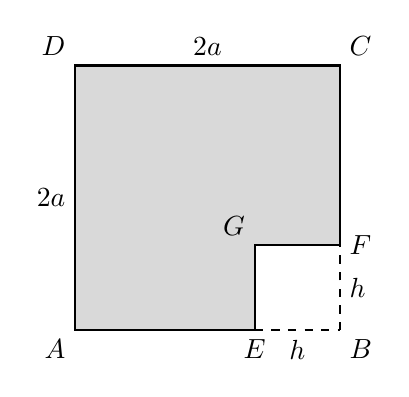
\begin{tikzpicture}[scale=1.2]
\def\aunit{1.4}
\def\hlen{0.9}
\pgfmathsetmacro{\side}{2*\aunit}

\coordinate (A) at (0,0);
\coordinate (B) at (\side,0);
\coordinate (C) at (\side,\side);
\coordinate (D) at (0,\side);
\coordinate (E) at ({\side-\hlen},0);
\coordinate (F) at (\side,\hlen);
\coordinate (G) at ({\side-\hlen},\hlen);

\fill[gray!30] (A) -- (E) -- (G) -- (F) -- (C) -- (D) -- cycle;
\draw[thick] (A) -- (E) -- (G) -- (F) -- (C) -- (D) -- cycle;
\draw[dashed, thick] (E) -- (B);
\draw[dashed, thick] (B) -- (F);

\node[below] at ($(E)!0.5!(B)$) {$h$};
\node[right] at ($(B)!0.5!(F)$) {$h$};
\node[above] at ($(D)!0.5!(C)$) {$2a$};
\node[left] at ($(A)!0.5!(D)$) {$2a$};

\node[below left] at (A) {$A$};
\node[below right] at (B) {$B$};
\node[above right] at (C) {$C$};
\node[above left] at (D) {$D$};
\node[below] at (E) {$E$};
\node[right] at (F) {$F$};
\node[above left] at (G) {$G$};
\end{tikzpicture}
\end{figure}


A uniform lamina is formed by removing the square $EBGF$ from a square lamina $ABCD$, where $AB=BC=CD=DA=2a$ and $EB=BF=h$, with $0<h<2a$ (see diagram). \\
\begin{enumerate}[label=\textbf{(\alph*)}]
  \item Find the distance of the centre of mass of the remaining lamina from $AD$ and from $AB$, giving your answers in terms of $a$ and $h$. \marks{5} \\
\end{enumerate}
The lamina is placed vertically on its edge $AE$ on a horizontal plane. \\
\begin{enumerate}[label=\textbf{(\alph*)}, resume]
  \item Find, in terms of $a$, the set of values of $h$ for which the lamina remains in equilibrium. \marks{3} \\
\end{enumerate}

\newpage

% ---- Question 7 ----
\questionitem
% [Source: _QBT__Centre_of_Mass_of_Polygonal_Laminae, Q7]

\begin{figure}[H]
    \centering
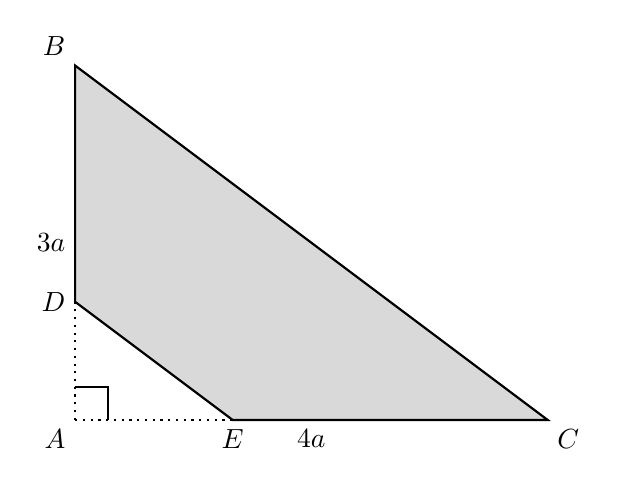
\begin{tikzpicture}[scale=1.5]
\def\xC{4}
\def\yB{3}
\def\kshown{3}
\pgfmathsetmacro{\t}{1/\kshown}

\coordinate (A) at (0,0);
\coordinate (B) at (0,\yB);
\coordinate (C) at (\xC,0);
\coordinate (D) at (0,{\yB*\t});
\coordinate (E) at ({\xC*\t},0);

\fill[gray!30] (D) -- (B) -- (C) -- (E) -- cycle;

\draw[thick] (D) -- (B) -- (C) -- (E) -- cycle;
\draw[dotted, thick] (A) -- (D);
\draw[dotted, thick] (A) -- (E);

\draw[thick] (0.28,0) -- (0.28,0.28) -- (0,0.28);

\node[below left] at (A) {$A$};
\node[above left] at (B) {$B$};
\node[below right] at (C) {$C$};
\node[left] at (D) {$D$};
\node[below] at (E) {$E$};
\node[left] at ($(A)!0.5!(B)$) {$3a$};
\node[below] at ($(A)!0.5!(C)$) {$4a$};
\end{tikzpicture}
\end{figure}


A uniform lamina is formed from the right-angled triangle $ABC$ by removing the triangle $ADE$, as shown in the diagram. The triangle $ABC$ has $AB=3a$, $AC=4a$ and $\angle BAC=90^\circ$. The point $D$ lies on $AB$ and satisfies $AD:AB=1:k$. The point $E$ lies on $AC$, and $DE$ is parallel to $BC$. \\
\begin{enumerate}[label=\textbf{(\alph*)}]
  \item Taking $A$ as the origin, with $AC$ as the $x$-axis and $AB$ as the $y$-axis, find the coordinates of the centre of mass of the remaining lamina $DBCE$ in terms of $a$ and $k$. \marks{4} \\
\end{enumerate}
When the lamina $DBCE$ is freely suspended from $C$, the edge $CE$ makes an angle $\theta$ with the downward vertical, where $\tan\theta=\dfrac{21}{52}$. \\
\begin{enumerate}[label=\textbf{(\alph*)}, resume]
  \item Find the value of $k$. \marks{3} \\
\end{enumerate}

\newpage

% ---- Question 8 ----
\questionitem
% [Source: _QBT__Centre_of_Mass_of_Polygonal_Laminae, Q8]

\begin{figure}[H]
    \centering
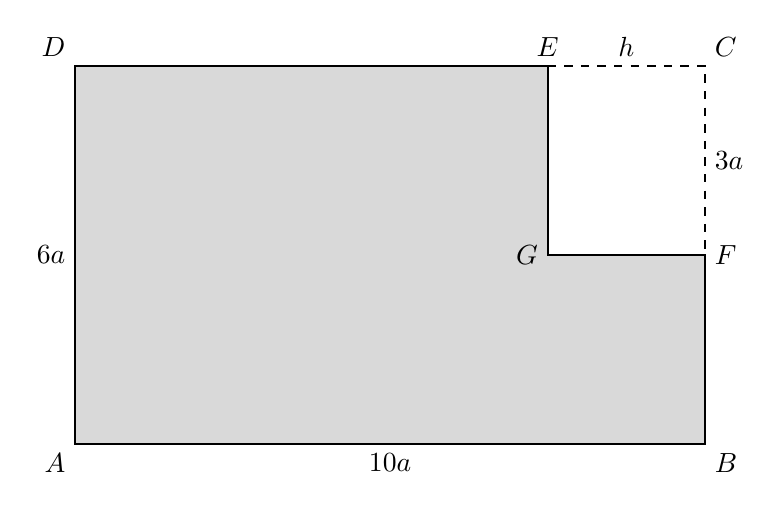
\begin{tikzpicture}[scale=0.8]
\def\W{10}
\def\H{6}
\def\k{3}
\def\h{2.5}
\coordinate (A) at (0,0);
\coordinate (B) at (\W,0);
\coordinate (C) at (\W,\H);
\coordinate (D) at (0,\H);
\coordinate (E) at ({\W-\h},\H);
\coordinate (F) at (\W,{\H-\k});
\coordinate (G) at ({\W-\h},{\H-\k});

\fill[gray!30] (A) -- (B) -- (F) -- (G) -- (E) -- (D) -- cycle;
\draw[thick] (A) -- (B) -- (F) -- (G) -- (E) -- (D) -- cycle;
\draw[dashed, thick] (E) -- (C) -- (F);

\node[below left] at (A) {$A$};
\node[below right] at (B) {$B$};
\node[above right] at (C) {$C$};
\node[above left] at (D) {$D$};
\node[above] at (E) {$E$};
\node[right] at (F) {$F$};
\node[left] at (G) {$G$};

\node[above] at ($(E)!0.5!(C)$) {$h$};
\node[right] at ($(C)!0.5!(F)$) {$3a$};
\node[below] at ($(A)!0.5!(B)$) {$10a$};
\node[left] at ($(A)!0.5!(D)$) {$6a$};
\end{tikzpicture}
\end{figure}


$ABCD$ is a uniform rectangular lamina with $AB=10a$ and $BC=6a$. Point $E$ lies on $DC$ with $CE=h$, where $0<h<10a$, and point $F$ lies on $BC$ with $CF=3a$. The rectangle $CEGF$ is removed, where $G$ is the fourth vertex of the rectangle (see diagram). \\
\begin{enumerate}[label=\textbf{(\alph*)}]
  \item Show that the distance of the centre of mass of the remaining lamina from $AD$ is
  \[
  \dfrac{h^2-20ah+200a^2}{2(20a-h)}
  \]
  and find a corresponding expression for the distance of the centre of mass from $AB$. \marks{5} \\
\end{enumerate}
When the lamina is suspended from the point $D$, the edge $DA$ makes an angle $\theta$ with the downward vertical, where $\tan\theta=\tfrac{13}{12}$. \\
\begin{enumerate}[label=\textbf{(\alph*)}, resume]
  \item Find, in terms of $a$, the two possible values of $h$. \marks{3} \\
\end{enumerate}

\newpage

% ---- Question 9 ----
\questionitem
% [Source: _QBT__Centre_of_Mass_of_Polygonal_Laminae, Q9]

\begin{figure}[H]
    \centering
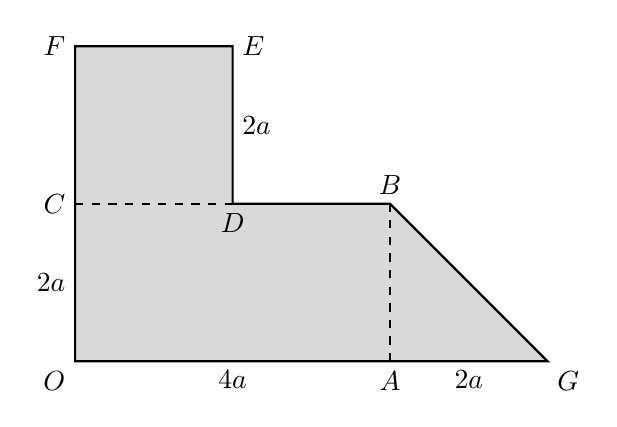
\begin{tikzpicture}[scale=1.0]
\def\w{4}
\def\h{2}
\def\s{2}

\coordinate (O) at (0,0);
\coordinate (A) at (\w,0);
\coordinate (G) at ({\w+\s},0);
\coordinate (B) at (\w,\h);
\coordinate (C) at (0,\h);
\coordinate (D) at (\s,\h);
\coordinate (E) at (\s,{\h+\s});
\coordinate (F) at (0,{\h+\s});

\fill[gray!30] (O) -- (A) -- (B) -- (C) -- cycle;
\fill[gray!30] (C) -- (D) -- (E) -- (F) -- cycle;
\fill[gray!30] (A) -- (G) -- (B) -- cycle;

\draw[thick] (O) -- (A) -- (G) -- (B) -- (D) -- (E) -- (F) -- (C) -- cycle;

\draw[dashed, thick] (A) -- (B);
\draw[dashed, thick] (C) -- (D);

\node[below] at ($(O)!0.5!(A)$) {$4a$};
\node[below] at ($(A)!0.5!(G)$) {$2a$};
\node[left] at ($(O)!0.5!(C)$) {$2a$};
\node[right] at ($(D)!0.5!(E)$) {$2a$};

\node[below left] at (O) {$O$};
\node[below] at (A) {$A$};
\node[below right] at (G) {$G$};
\node[above] at (B) {$B$};
\node[left] at (C) {$C$};
\node[below] at (D) {$D$};
\node[right] at (E) {$E$};
\node[left] at (F) {$F$};
\end{tikzpicture}
\end{figure}


The uniform plane lamina shown in the diagram is formed from the rectangle $OABC$, the square $CDEF$ and the triangle $ABG$. The rectangle has dimensions $4a$ by $2a$, the square has side $2a$ and $AG=2a$. Take $O$ as the origin, with $OA$ as the positive $x$-axis and $OC$ as the positive $y$-axis. \\

In part (a) you may use, without proof, any of the centre of mass formulae given in the formulae booklet. \\
\begin{enumerate}[label=\textbf{(\alph*)}]
  \item Show that the distance of the centre of mass of triangle $ABG$ from $AB$ is $\dfrac{2a}{3}$. \marks{3} \\
  \item Find the coordinates of the centre of mass of the lamina. \marks{4} \\
\end{enumerate}
The lamina is freely suspended from $F$ and hangs in equilibrium with $FC$ at an angle $\theta^\circ$ to the downward vertical. \\
\begin{enumerate}[label=\textbf{(\alph*)}, resume]
  \item Find the value of $\theta$. \marks{4} \\
\end{enumerate}

\newpage

% ---- Question 10 ----
\questionitem
% [Source: _QBT__Centre_of_Mass_of_Polygonal_Laminae, Q10]

\begin{figure}[H]
    \centering
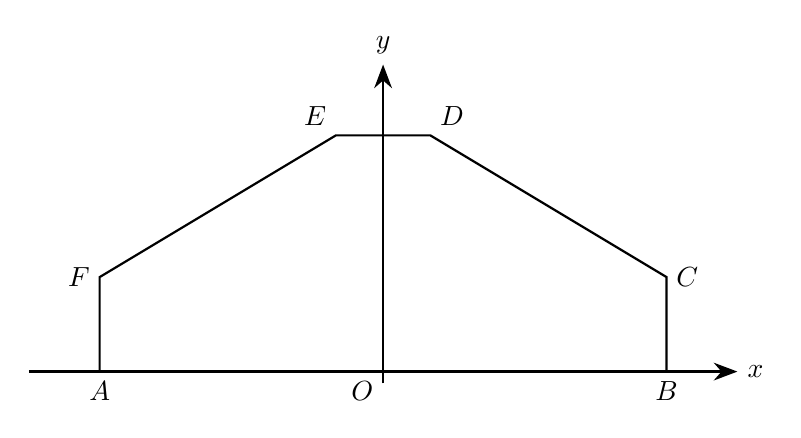
\begin{tikzpicture}[x=0.03cm,y=0.03cm]
\coordinate (O) at (0,0);
\coordinate (A) at (-120,0);
\coordinate (B) at (120,0);
\coordinate (C) at (120,40);
\coordinate (D) at (20,100);
\coordinate (E) at (-20,100);
\coordinate (F) at (-120,40);
\coordinate (X) at (150,0);
\coordinate (Y) at (0,130);

\draw[-{Stealth[length=3mm]}, thick] (-150,0) -- (X) node[right] {$x$};
\draw[-{Stealth[length=3mm]}, thick] (0,-5) -- (Y) node[above] {$y$};
\draw[thick] (A) -- (B) -- (C) -- (D) -- (E) -- (F) -- cycle;

\node[below] at (A) {$A$};
\node[below] at (B) {$B$};
\node[right] at (C) {$C$};
\node[above right] at (D) {$D$};
\node[above left] at (E) {$E$};
\node[left] at (F) {$F$};
\node[below left] at (O) {$O$};
\end{tikzpicture}
\end{figure}


A uniform lamina $ABCDEF$ is in the shape of the hexagon shown in the diagram. In a coordinate system with origin $O$, the vertices have coordinates $A(-120,0)$, $B(120,0)$, $C(120,40)$, $D(20,100)$, $E(-20,100)$ and $F(-120,40)$. The units of the axes are centimetres. \\

The centre of mass of the lamina lies at $(\bar{x},\bar{y})$. \\
\begin{enumerate}[label=\textbf{(\alph*)}]
  \item Use symmetry to write down $\bar{x}$ and show that $\bar{y}=40$. \marks{5} \\
\end{enumerate}
The lamina is placed horizontally so that it rests on three supports, whose points of contact are at $D$, $E$ and $G$, where $G$ lies on the edge $AB$ and has coordinates $(g,0)$. \\
\begin{enumerate}[label=\textbf{(\alph*)}, resume]
  \item Determine the range of values of $g$ for the lamina to rest in equilibrium. \marks{3} \\
\end{enumerate}
It is now given that $g=8$, and that the lamina has weight $100\mathrm{N}$. \\
\begin{enumerate}[label=\textbf{(\alph*)}, resume]
  \item Determine the forces exerted on the lamina by each of the supports at $D$, $E$ and $G$. \marks{4} \\
\end{enumerate}

\end{enumerate}
\end{document}
